%!TEX root = ../main.tex
\chapter{Validation of the time calibration}
\label{chap:TimingValidation}

It is necessary to perform a validation of the timing calibration (see chapter \ref{chap:TimingCalib}). The recorded electron data is used because electromagnetic showers are quasi-instantaneous and are perfect to validate the time calibration. The selection applied to the electron datasets is described in section \ref{subsec:elec_sel}. The same calibration constants and correction constants determined from the muon data are applied to the electron data.

\section{Time of the first hit for electrons}

The time of the first hit for 20 GeV electrons applying the calibration constants obtained from the muon data is shown in figure \ref{fig:Timing_electrons}. In addition, the distribution is compared to the time distribution from the muon data.

The peak of the electron time distribution in figure \ref{fig:Timing_electrons} is shifted to the left by around 10 ns. This time offset is expected due to a change in the trigger configuration (see section \ref{sec:TBsetup}). This offset is consistent with the difference between the trigger configurations in cable length to route the trigger signal.

Moreover, the time distribution of electrons presents a large tail to the right and is much wider than the one for muons. This could be related to the number of hits which is much higher in an electromagnetic shower than from a muon and also that the deposited energy in a single cell can be over 100 MIPs (see figure \ref{fig:eHitVal}).

\begin{figure}[htbp!]
	\centering
	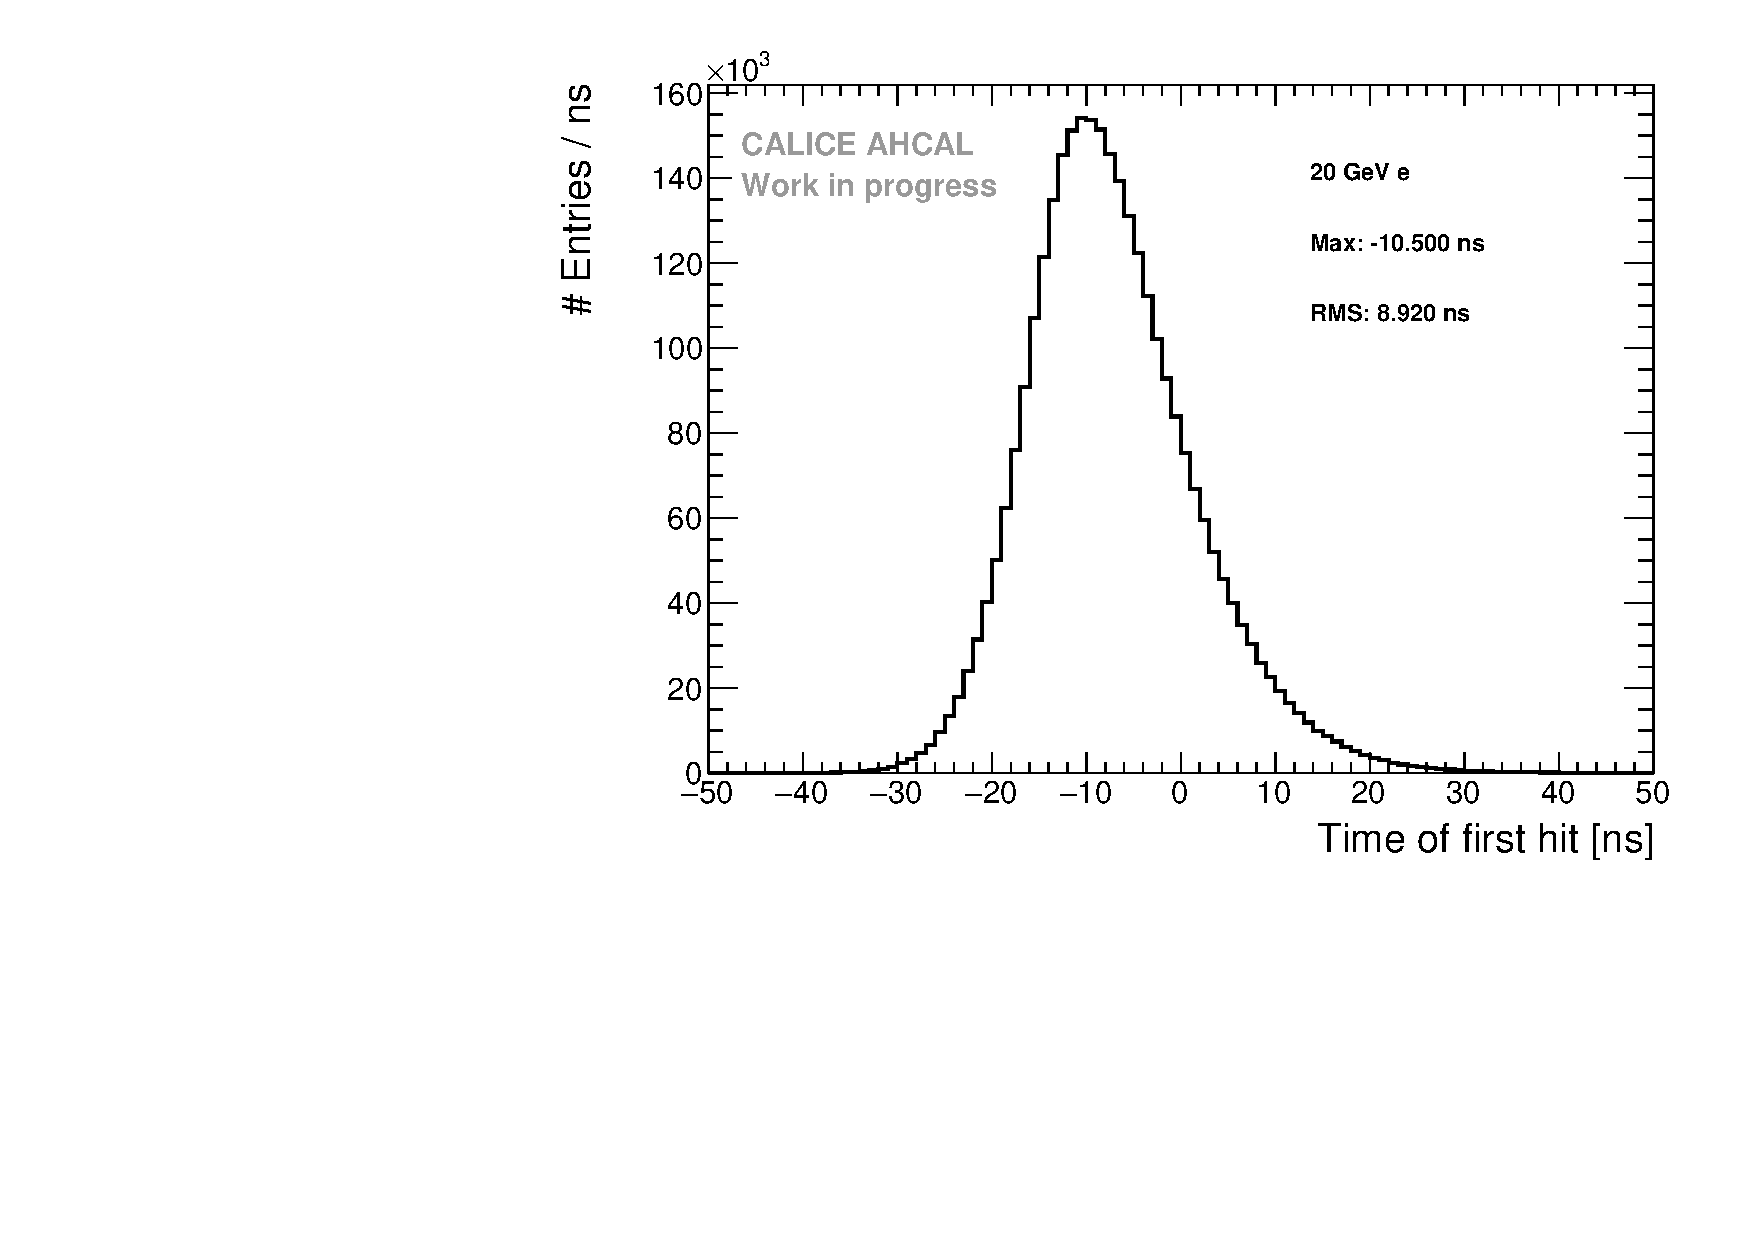
\includegraphics[width=0.6\textwidth]{../Thesis_Plots/Timing/Electrons/Plots/Timing_AllLayers_AfterMuons.pdf}
	\caption{Time of the first hit distribution for 20 GeV electrons after applying the calibration constants extracted from the muon data. The blue distribution represents the time of first hit distribution obtained with muons.}
	\label{fig:Timing_electrons}
\end{figure}

\section{Effect of the number of triggered channels on the time distribution}
\label{subsec:ped_shift}

For the energy measurement, there is a known and well understood feature of the SPIROC chip \cite{Hartbrich2012}, that induces a shift in the baseline of the ADC signal. This feature may be also present for the timing measurement. Since it is a priori not clear if the effect depends on the number of triggered channels \textit{in a chip} or the energy sum \textit{in a chip}, the time correction has been checked using both variables. It turned out that the time correction as a function of the number of triggered channels over 0.5 MIP in a chip give better results than the time correction as a function of the energy sum in a chip. This is not totally understood why. Both variables are correlated and it may be due to the fact that the number of triggered channels is a direct variable from the hardware compared to the energy sum which is interpreted from the charge stored by a chip.

The mean time of first hit as a function of the number of triggered channels over 0.5 MIP in a chip is shown in figure \ref{fig:nhits_profile}. The effect on the measured hit time can be very large, a correction up to 30-40 ns can be necessary to the data for a high number (15-20) of triggered channels above 0.5 MIP in a chip. The cause of the observed effect is most likely due to an element in the chip called a \textit{delay box} that gets unstable with a high charge going through the chip. This chip element is responsible for the hold signal of the TDC ramp in the chip. The hold signal is delayed, and thus a higher TDC ramp value than the one expected is sampled.

\begin{figure}[htbp!]
	\begin{subfigure}[t]{0.5\textwidth}
		\centering
		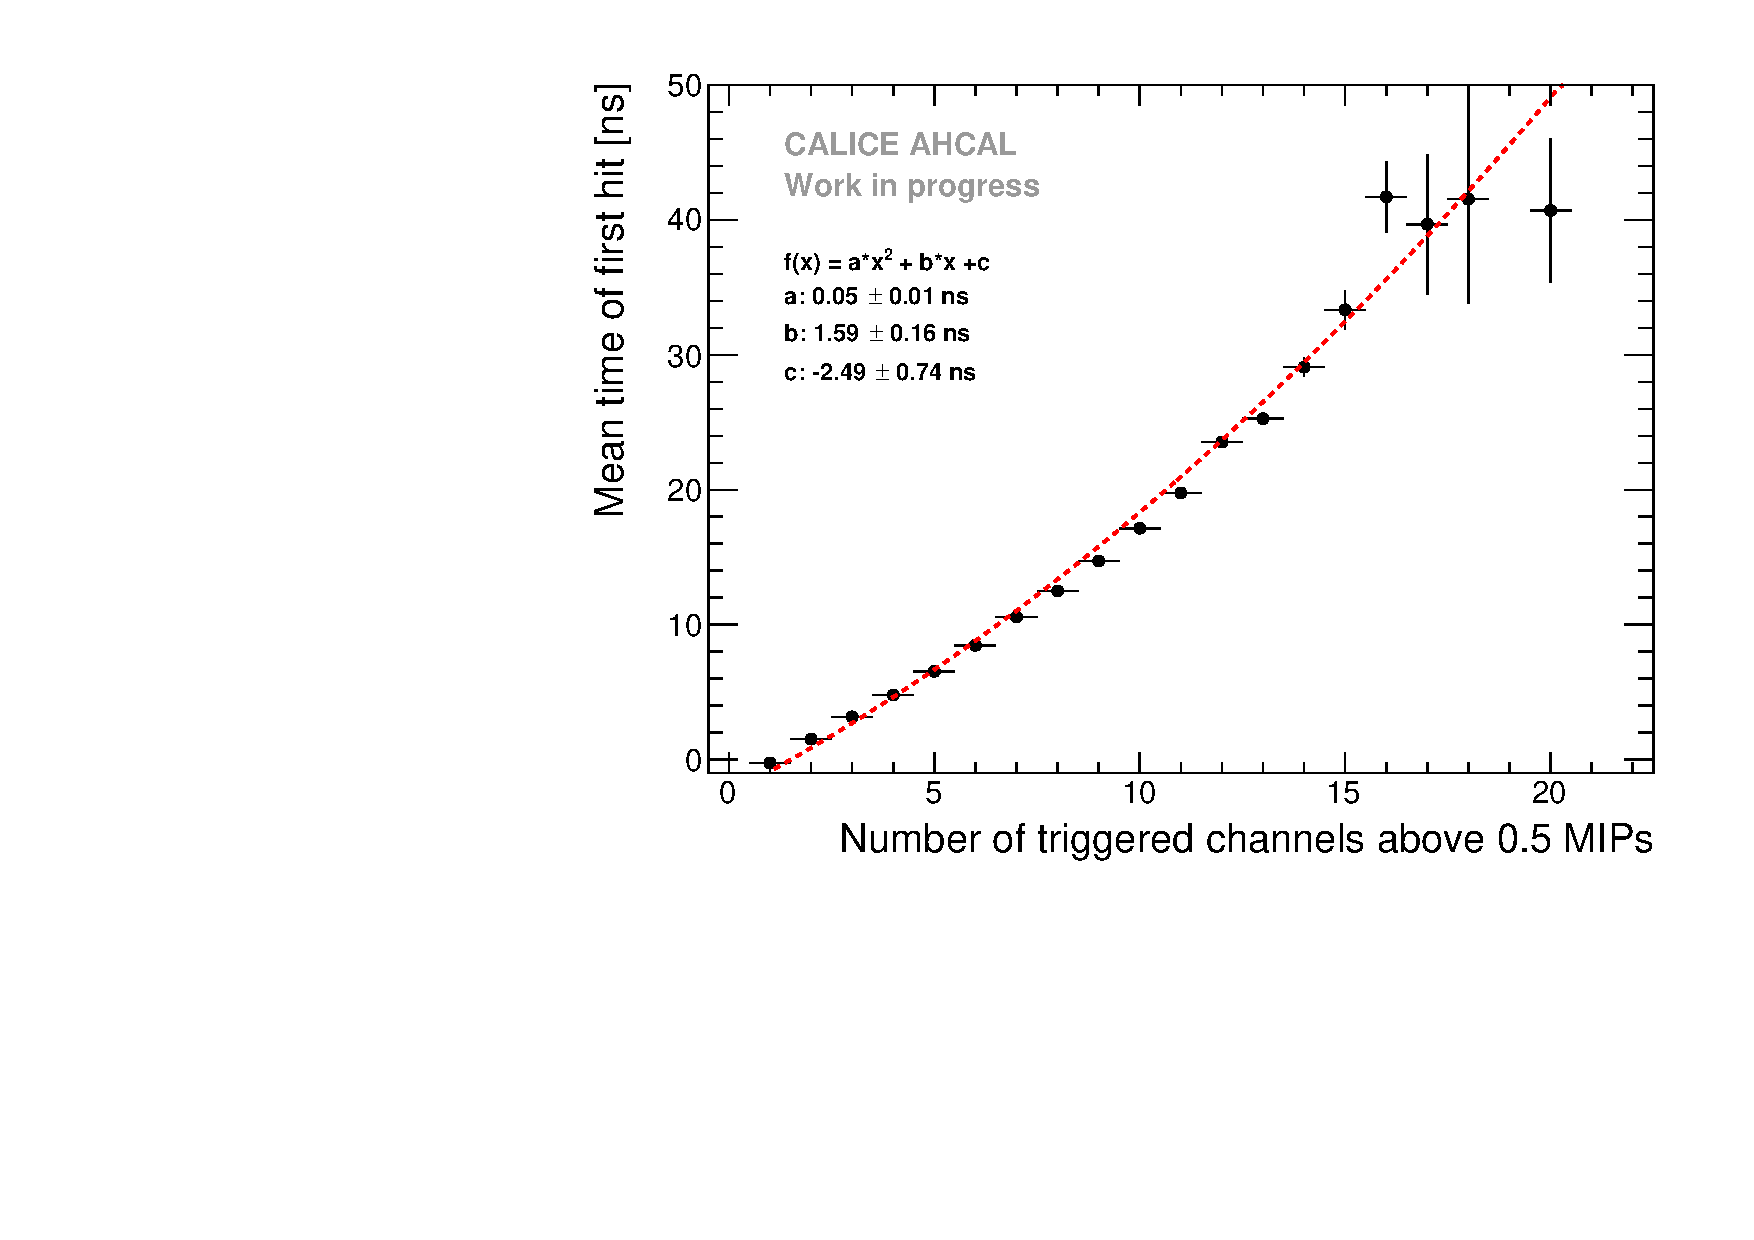
\includegraphics[width=1\textwidth]{../Thesis_Plots/Timing/Electrons/Plots/NumberHits_Dependance_AllEnergies.pdf}
		\caption{}\label{fig:nhits_profile}
	\end{subfigure}
	\hfill
	\begin{subfigure}[t]{0.5\textwidth}
		\centering
		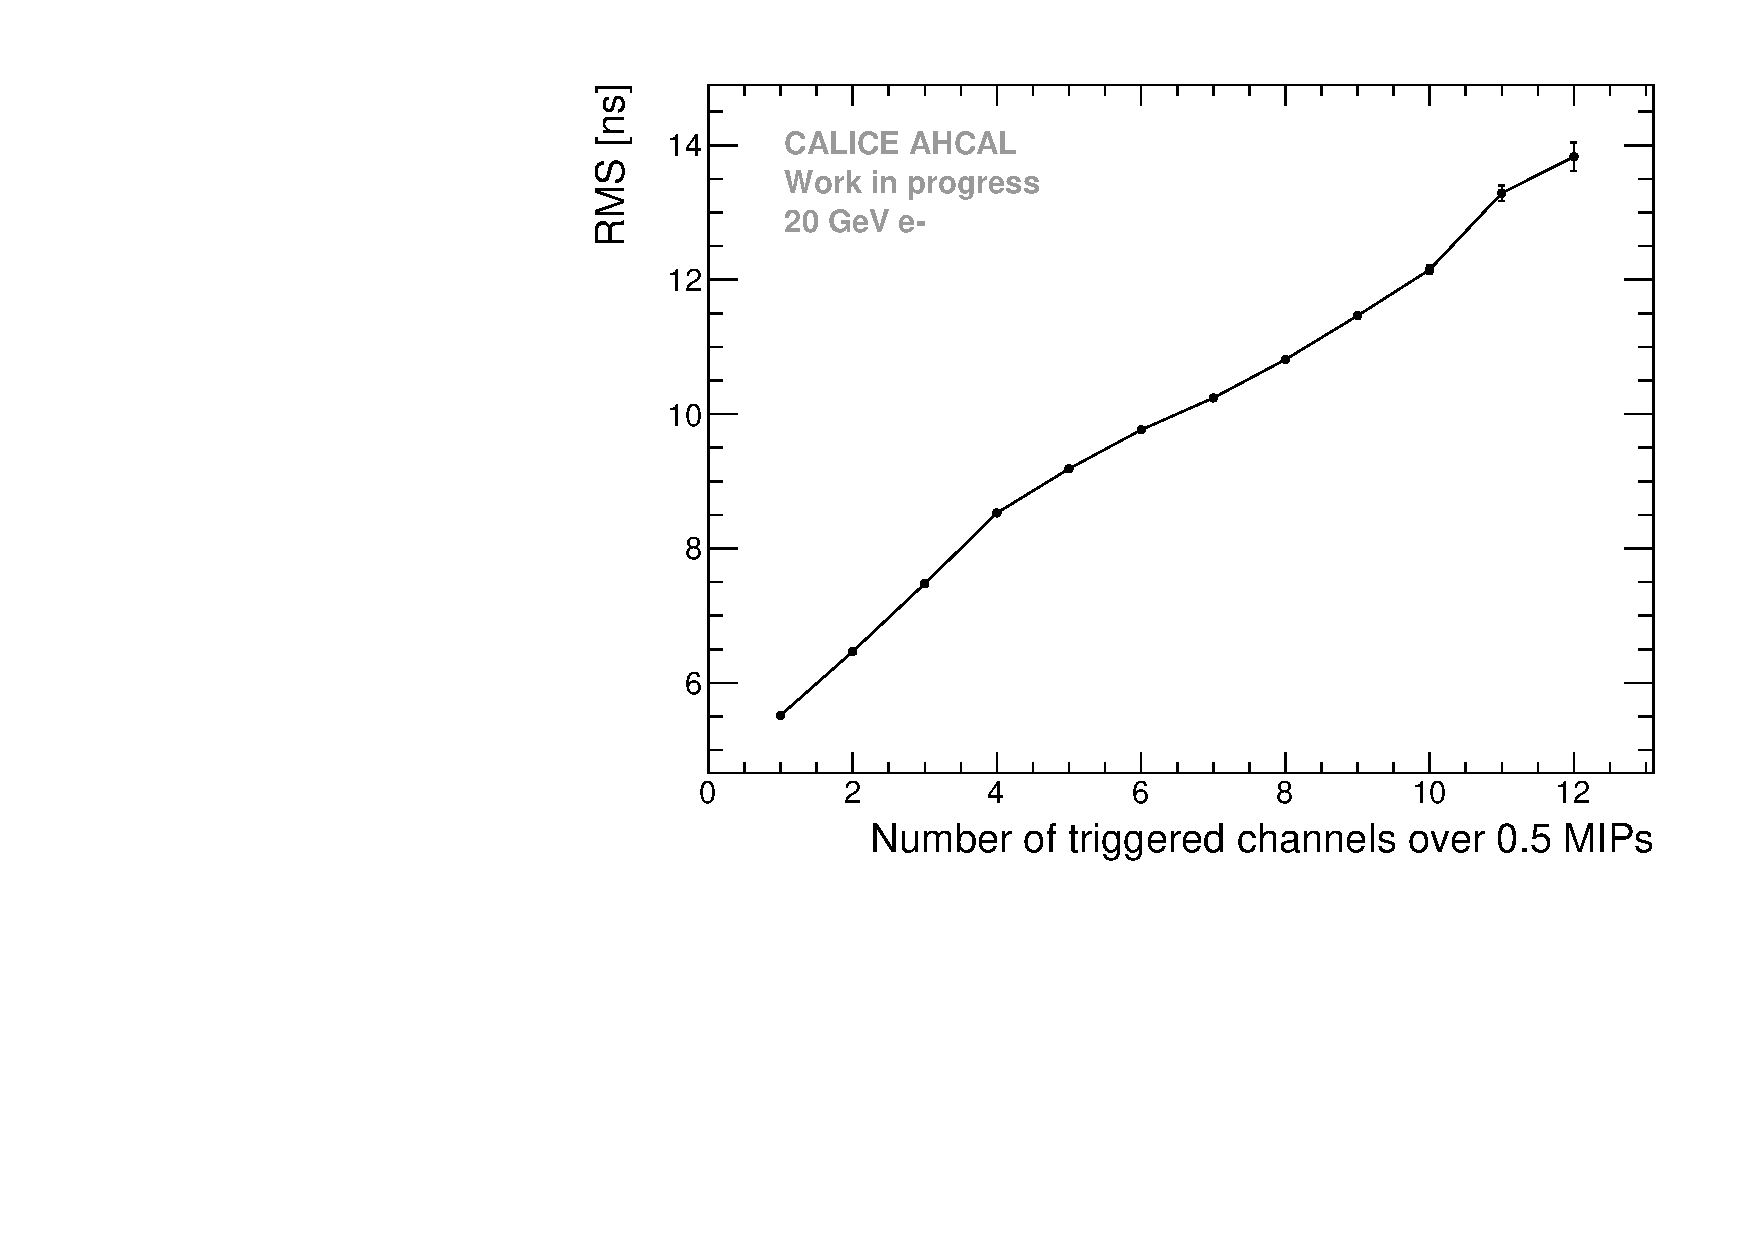
\includegraphics[width=1\textwidth]{../Thesis_Plots/Timing/Electrons/Plots/ParametrisationPedestalShift_20GeV.pdf}
		\caption{}\label{fig:RMS_nHits}
	\end{subfigure}
	\caption{\subref{fig:nhits_profile}) Mean time of the first hit as a function of the number of triggered channels above 0.5 MIP in a chip. The mean time shift upwards with the increase of triggers leading to large tails in the time distribution. The plot is obtained by combining all electron energies and a second order polynomial fit is done. \subref{fig:RMS_nHits}) The RMS of the time of first hit distribution as a function of the number of triggered channels above 0.5 MIP in a chip for 20 GeV electrons. The RMS of the time distribution can increase up to 10-15 ns for a high number of triggered channels in a chip.}
\end{figure}

The time correction parameters are determined by a $2^{nd}$ order polynomial fit to the data. In order to determine a reliable time correction, the time correction parameters are determined combining all the electron data. This effect is chip-dependent and the parameters for the correction may differ from chip to chip. However, the limited amount of data does not allow to determine a correction function for each chip. Therefore, a global function is used to correct the time in the data.

The figure \ref{fig:RMS_nHits} shows the RMS of the time distribution as a function of the number of triggered channels over 0.5 MIP in a chip. The width of the time distribution increases with a higher number of triggered channels in a chip. Therefore, the time resolution of the AHCAL is dependent on the number of triggered channels in a chip, thus the number of hits in the calorimeter. It is expected that the time resolution increases as a function of the electron beam energy as the number of hits in a EM shower is proportional to its energy. Moreover, the timing resolution is expected to be slightly dependent on the electron beam profile that affects directly the number of triggered channels in a chip.

As expected, if a single channel in a chip triggers, the RMS of the time distribution is close to the time resolution for muons as shown in figure \ref{fig:RMS_nHits}.

\section{Time of the first hit after correction}
\label{subsec:Electron_Final}

After applying the correction as function of the number of triggered channels in a chip, the distribution of the time of the first for 20 GeV electrons has been investigated as shown in figure \ref{fig:timing_electrons_corr}. The correction improves the RMS of the distribution by around 12.1\%, as well as the distribution appears more Gaussian-like.

However, there is still a discrepancy of around 33.7\% with the time resolution obtained with muons of around 5.36 ns (see section \ref{subsec:Muon_final}). This is because of the increase of the RMS of the time distribution as a function of the number of triggered channels in a chip as seen in figure \ref{fig:RMS_nHits}. The increase of the RMS can't be corrected unlike the mean of the time distribution.

In order for the simulation to match the data, the increase of the width of the time distribution has to be parametrized from the data. More details about the parametrization implementation in the simulation are in the appendix \ref{appendix:ped_shift}.

\begin{figure}[htbp!]
	\begin{subfigure}[t]{0.5\textwidth}
		\centering
		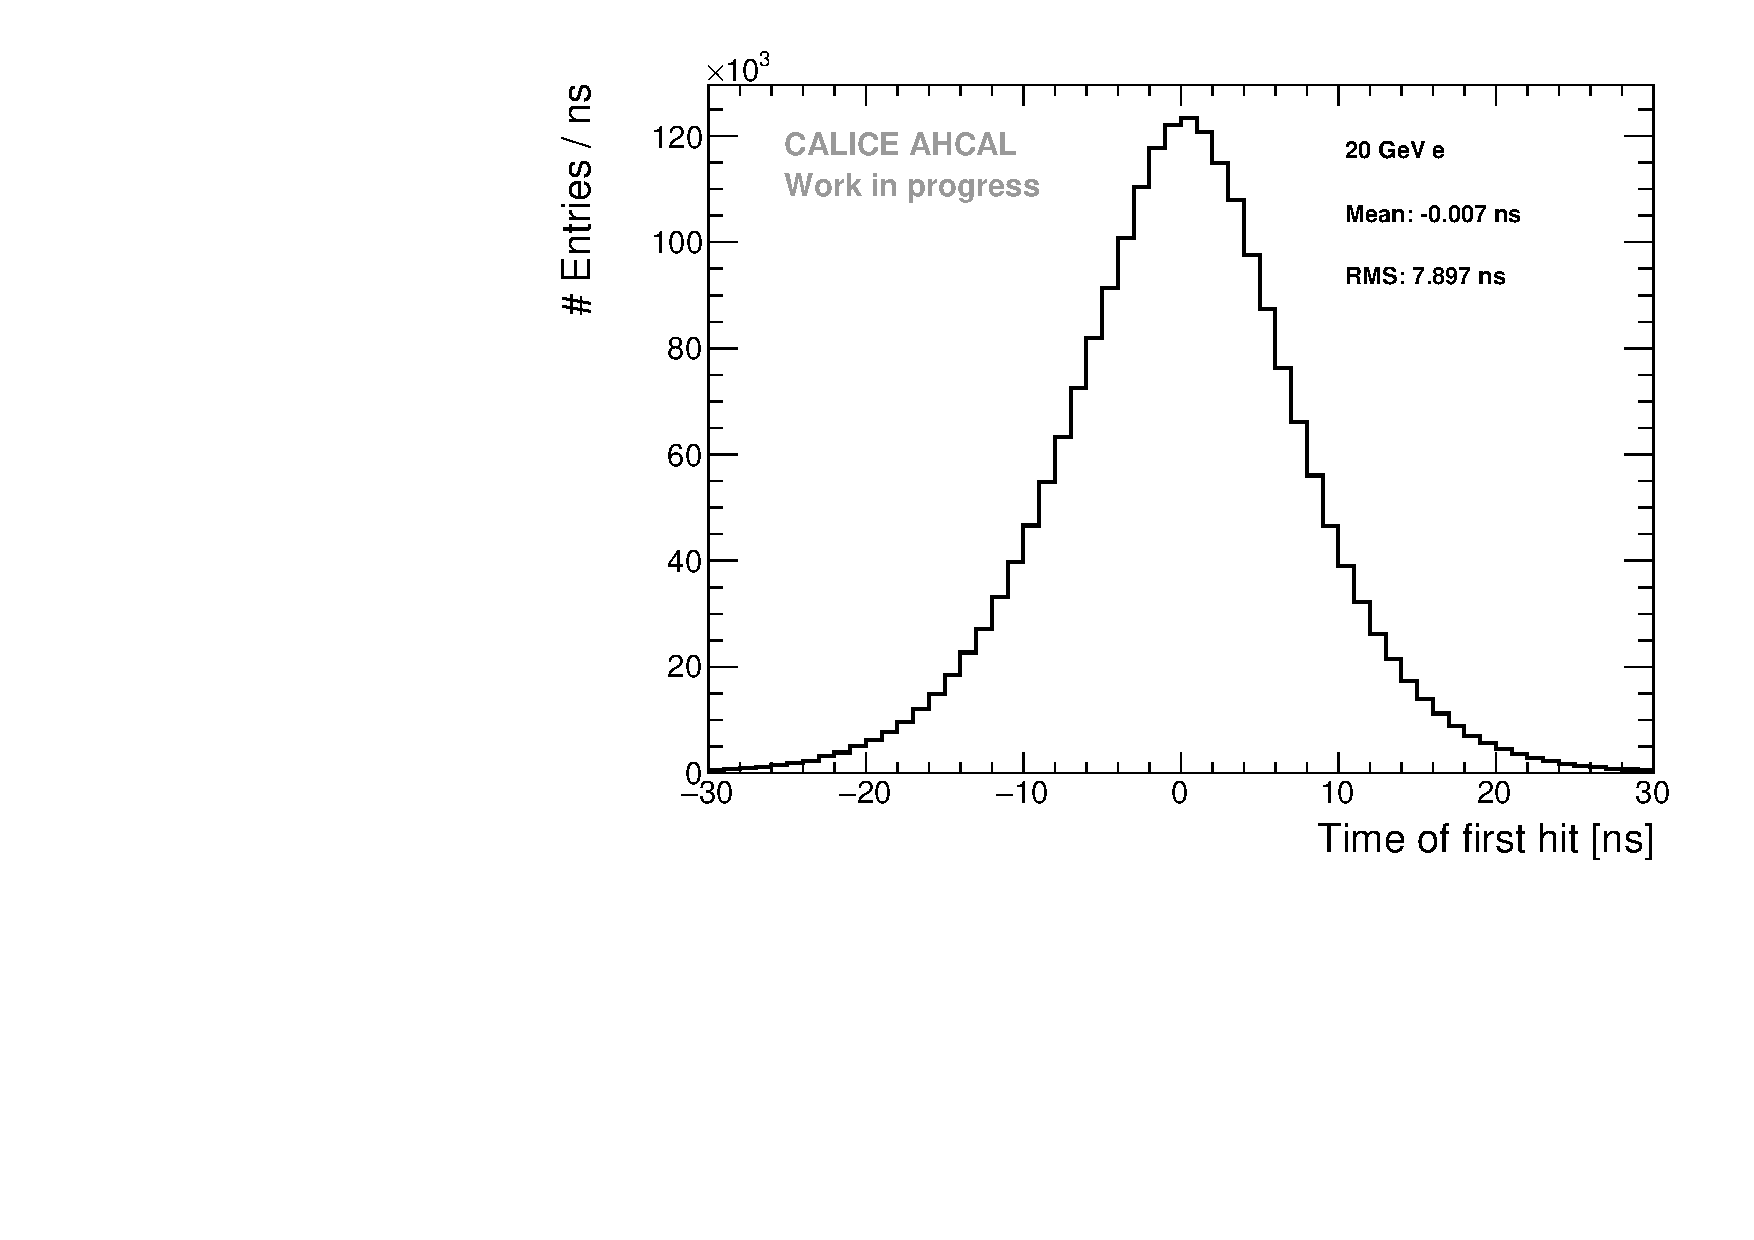
\includegraphics[width=1\textwidth]{../Thesis_Plots/Timing/Electrons/Plots/Timing_AllLayers_20GeV.pdf}
		\caption{}\label{fig:timing_electrons_corr}
	\end{subfigure}
	\hfill
	\begin{subfigure}[t]{0.5\textwidth}
		\centering
		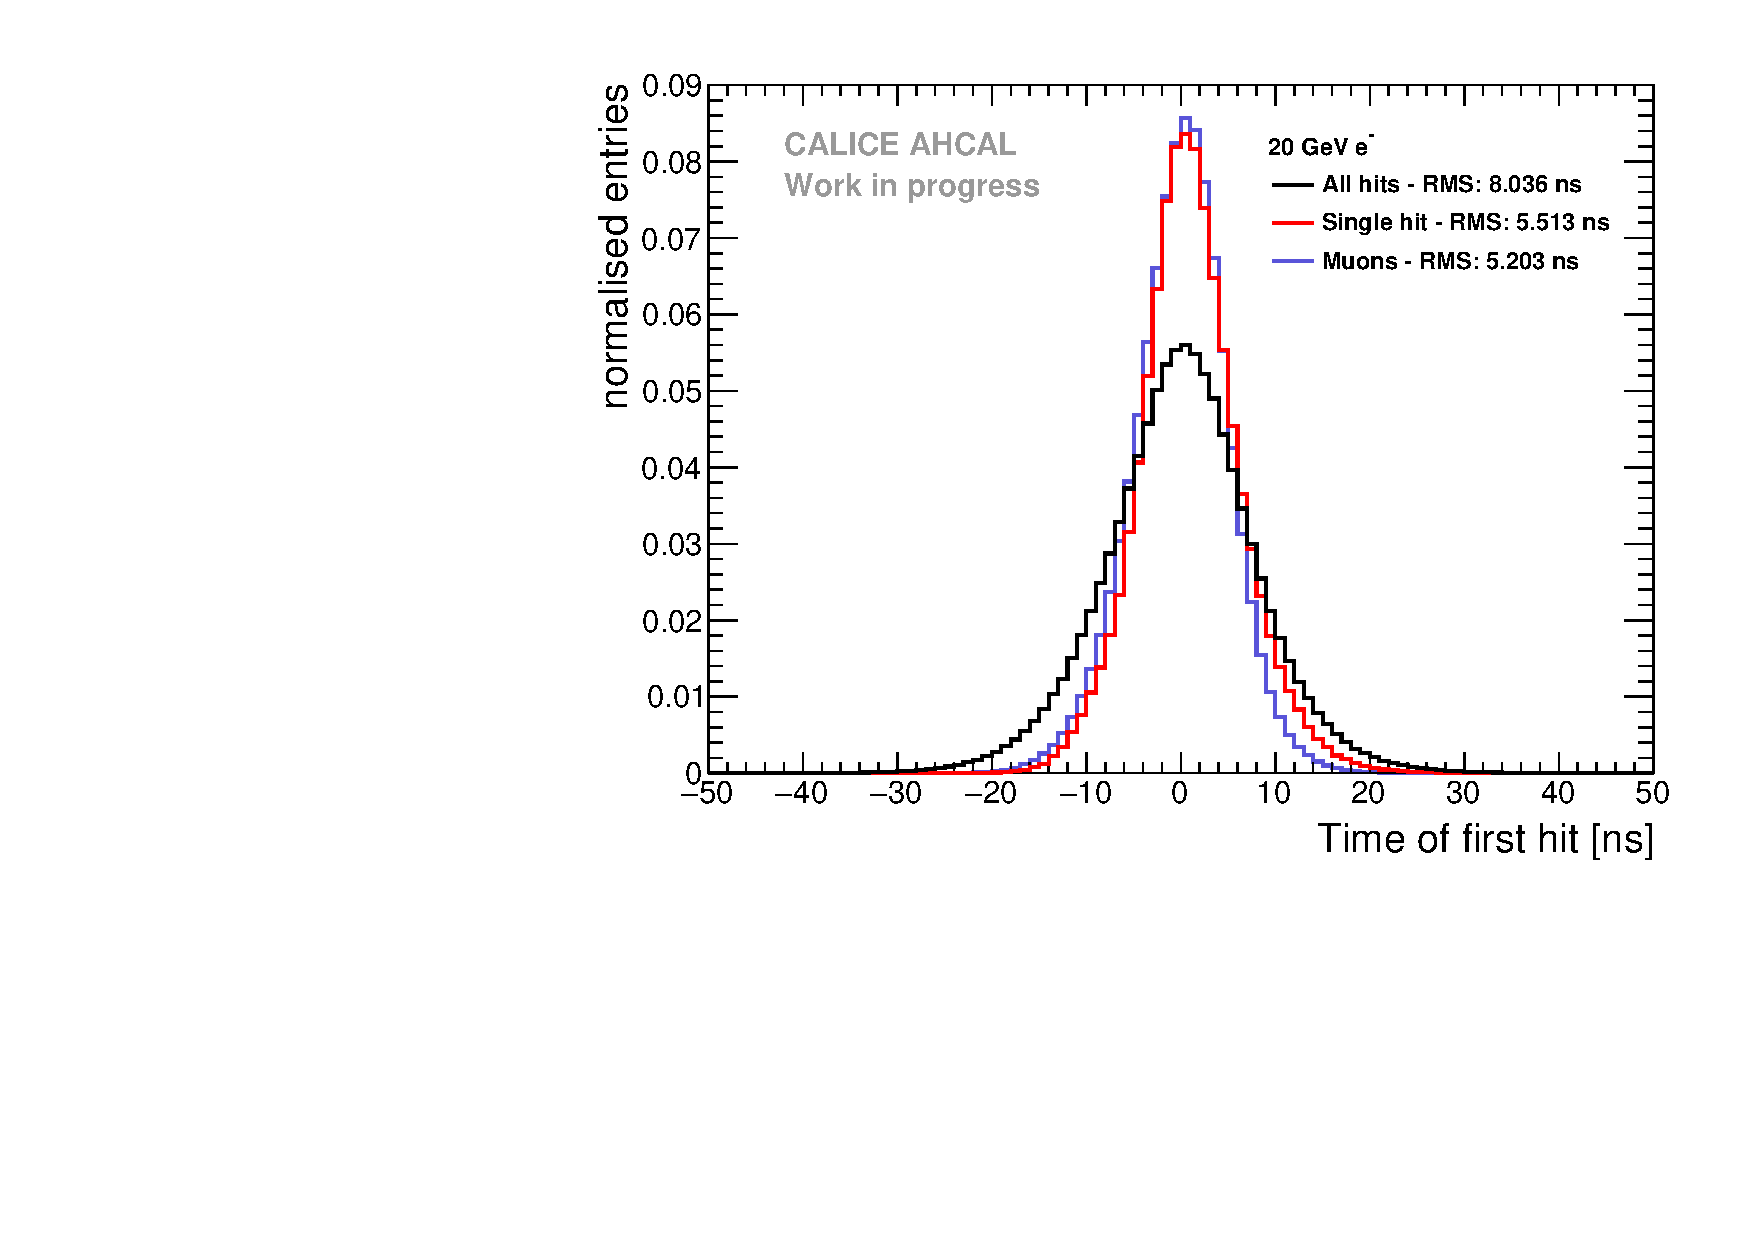
\includegraphics[width=1\textwidth]{../Thesis_Plots/Timing/Electrons/Plots/ComparisonAll_ElectronsSingleHit.pdf}
		\caption{}\label{fig:timing_electron_muon_comp}
	\end{subfigure}
	\caption{\subref{fig:timing_electrons_corr}) Time of the first hit distribution for 20 GeV electrons after the number of triggered channel correction, $\mu$ = -0.018 ns, RMS = 7.84 ns. \subref{fig:timing_electron_muon_comp}) Comparison of the 20 GeV electron sample with the muon time distribution for the time of first hit distribution. The time distribution is very similar to the distribution obtained with muons if only events in which only single hits in a chip are taken.}
\end{figure}

A comparison with the muon data has been done in order to further cross-check the calibration as well as the correction. The comparison is shown in figure \ref{fig:timing_electron_muon_comp}. If only event in which single hits in a chip are taken, the time resolution obtained is very similar to the time resolution observed with muons. The difference is around 5.2\%.

\begin{figure}[htbp!]
	\centering
	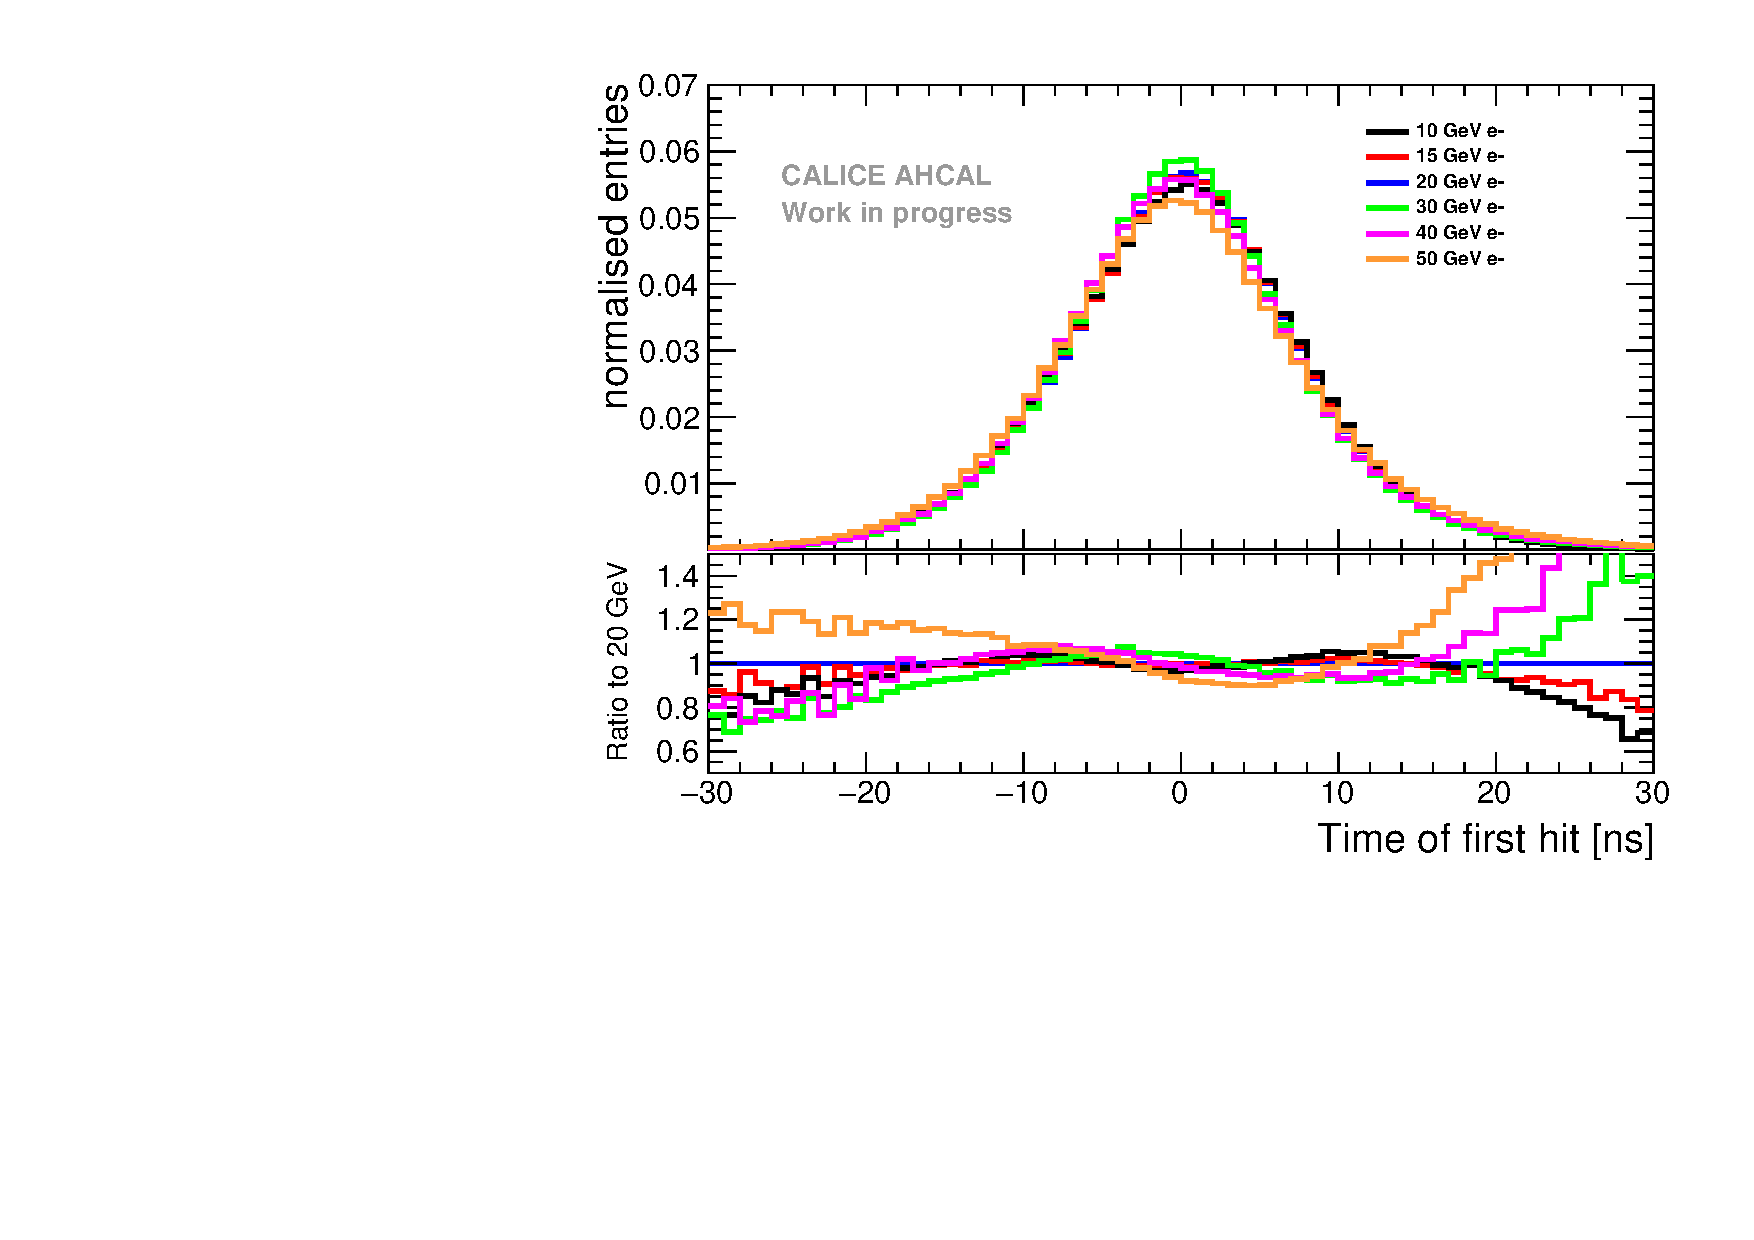
\includegraphics[width=0.6\textwidth]{../Thesis_Plots/Timing/Electrons/Plots/ComparisonDataEnergies.pdf}
	\caption{Comparison of the time of first hit distribution for all electron energies.}
	\label{fig:all_electron_energies}
\end{figure}

All electron runs (see section \ref{sec:TimingIntro}) have been carefully checked to validate the correction and the timing calibration. The figure \ref{fig:all_electron_energies} shows the comparison from 10 GeV to 50 GeV. The time distributions are in good agreement for all energies. The mean of the time distributions is very similar for all energies. The RMS of the time distributions varies between 7.86 ns at 10 GeV and 8.50 ns at 50 GeV corresponding to an increase of 8.1\%.

\section{Influence of the detector inhomogeneity}
\label{subsec:det_inhomo}

A study has been performed to estimate the influence of the detector inhomogeneity in space on timing. For this, only events in which the center of gravity in x and y is within the four center tiles of the detector are selected. Each of the four tiles is study separately. This has been performed for 10 and 50 GeV electron beam energy. The difference between the distributions helps to estimate the systematic uncertainty due to the inhomogeneity of the detector to which electrons are very sensitive to.

\begin{figure}[htbp!]
	\begin{subfigure}[t]{0.5\textwidth}
		\centering
		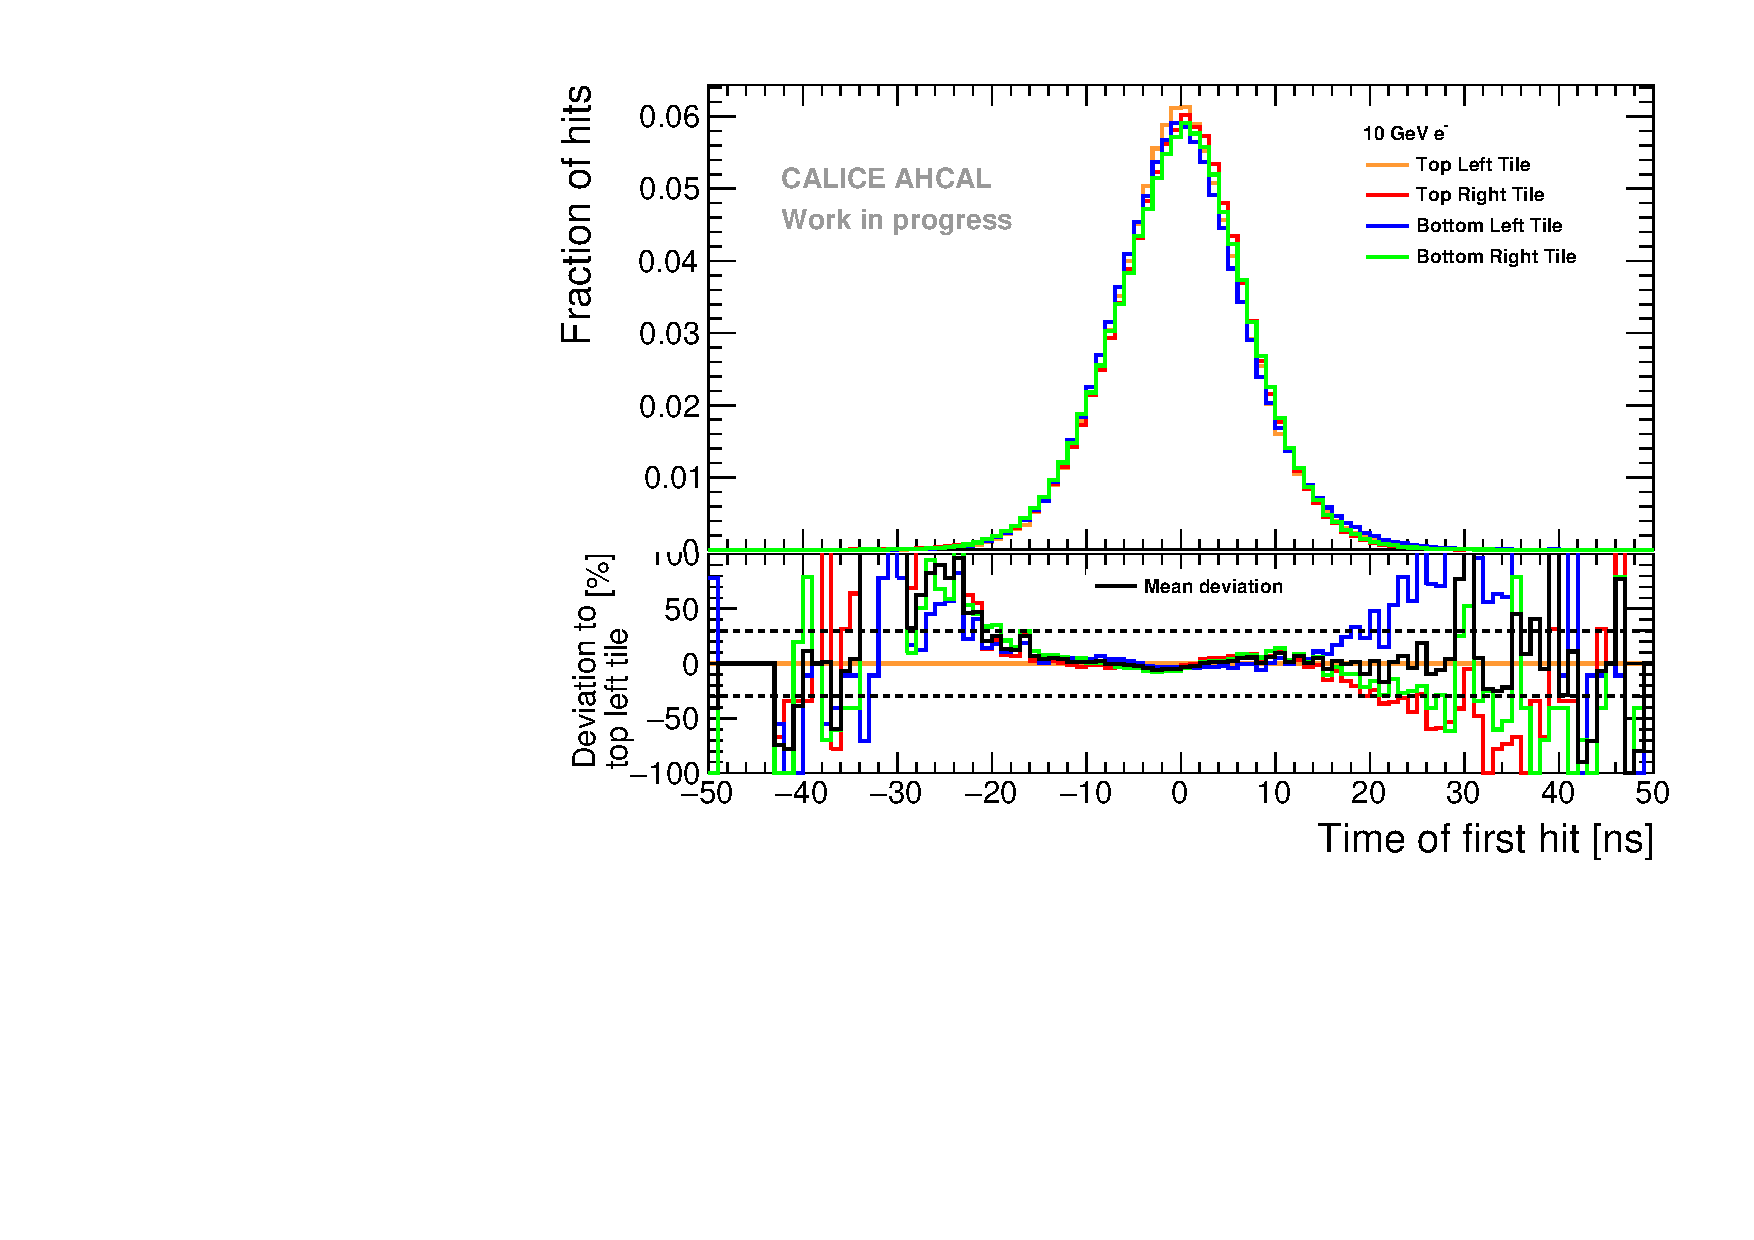
\includegraphics[width=1\textwidth]{../Thesis_Plots/Timing/Electrons/Plots/Systematic_Inhomogeneity_10GeV.pdf}
		\caption{}\label{fig:timing_inhomo_10GeV}
	\end{subfigure}
	\hfill
	\begin{subfigure}[t]{0.5\textwidth}
		\centering
		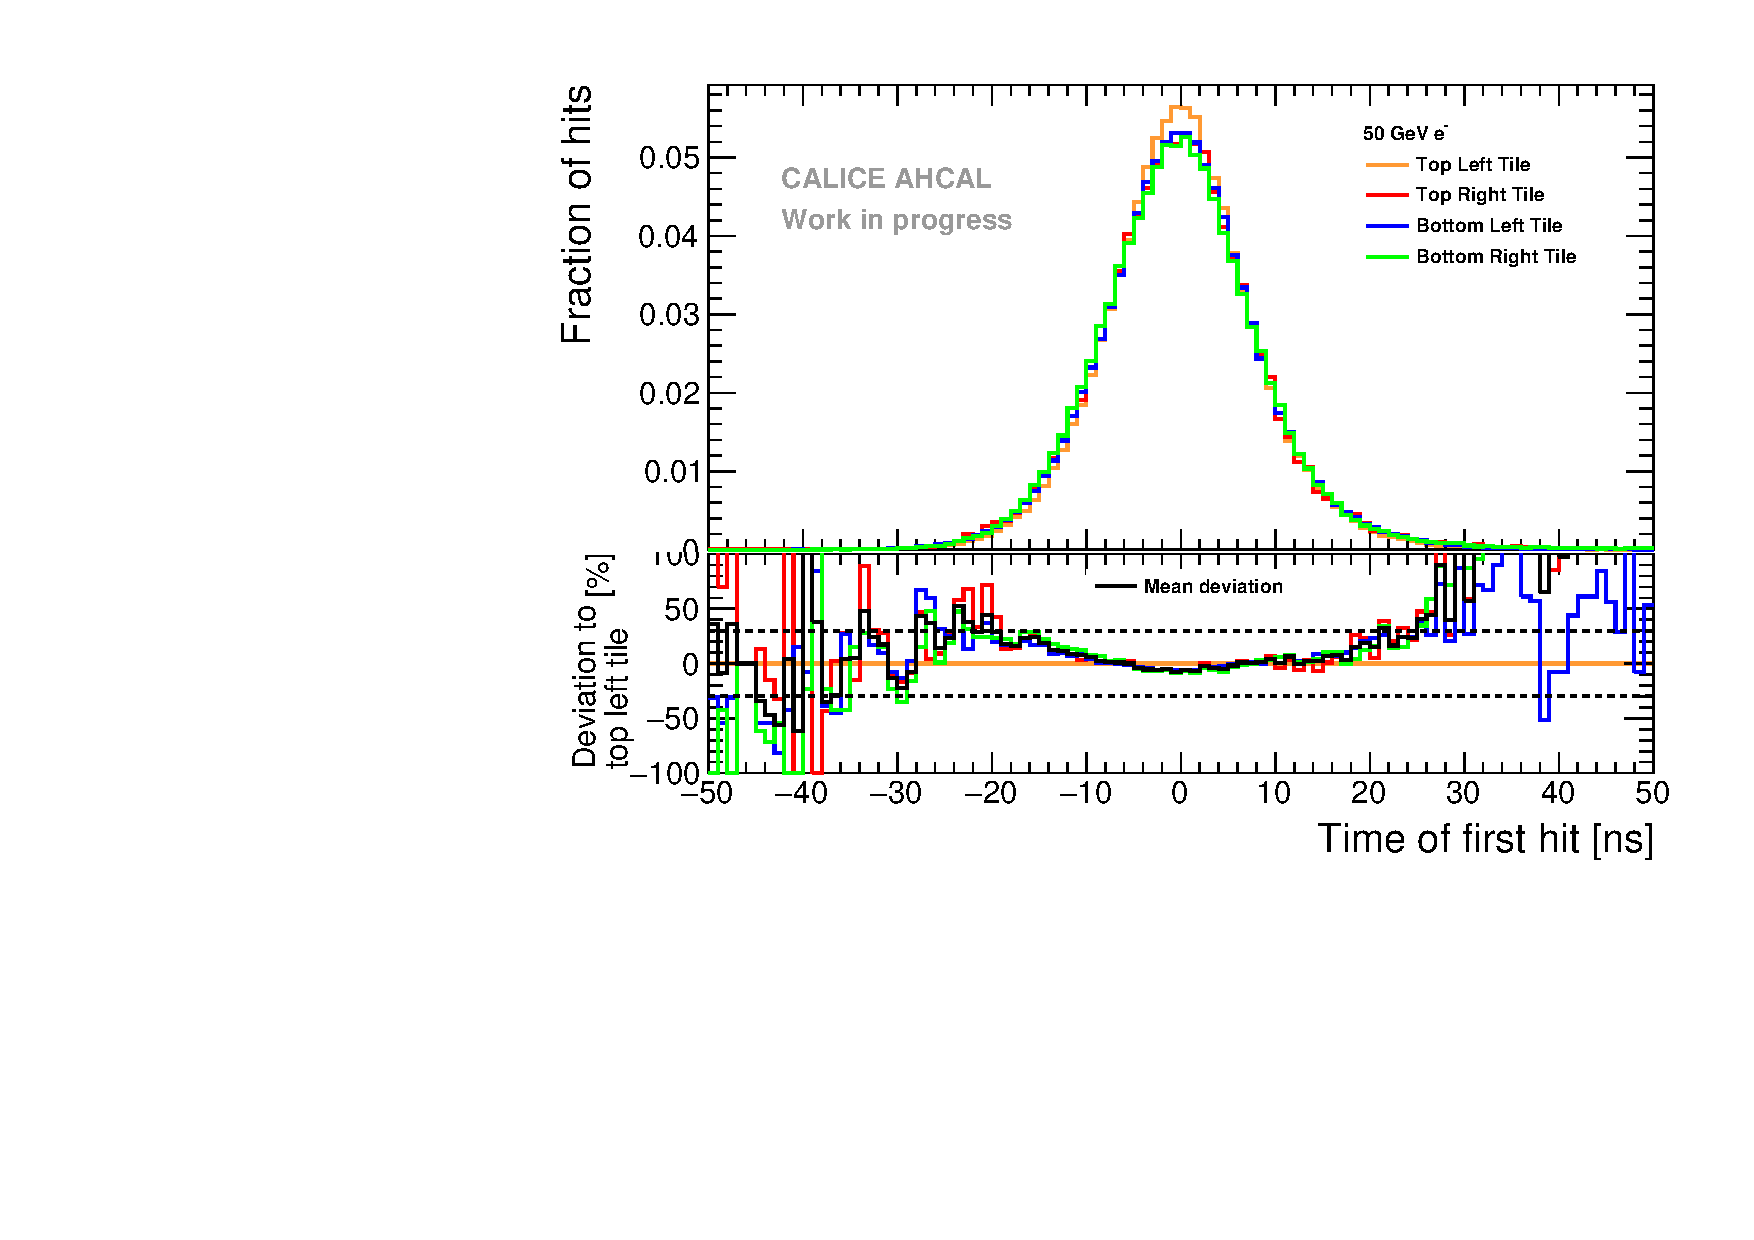
\includegraphics[width=1\textwidth]{../Thesis_Plots/Timing/Electrons/Plots/Systematic_Inhomogeneity_50GeV.pdf}
		\caption{}\label{fig:timing_inhomo_50GeV}
	\end{subfigure}
	\caption{\subref{fig:timing_inhomo_10GeV}) Time of the first hit distribution for all four middle tiles with 10 GeV electron beam. \subref{fig:timing_inhomo_50GeV}) Time of the first hit distribution for all four middle tiles with 50 GeV electron beam. All distribution are within 10-20\% in the core.}
\end{figure}

The figures \ref{fig:timing_inhomo_10GeV} and \ref{fig:timing_inhomo_50GeV} show the time distribution for each of the four tiles at 10 and 50 GeV respectively. The ratio shown is compared to the top left center tile. At 50 GeV, the mean of the distributions vary between -0.02 ns and -0.13 ns. The RMS of the distributions vary between 7.86 ns and 8.33 ns corresponding to an increase of 6\%. For both energies, the distributions are within a 10-20\% agreement in the region between -30 ns and 30 ns.

\section{Transportability of the calibration}

A check on the validity of the calibration for other data-taking periods has been performed on another dataset from a testbeam at DESY II in May 2016. The goal was to understand how transportable is the time calibration. The setup was composed of the same four big layers used at CERN in July 2015. In order to have enough hits in all layers, an aluminum absorber of 3 $X_{0}$ was placed in front of the detector in a 3 GeV electron beam.

The same calibration constants determined from the CERN muon and electron data were used. Just a re-calibration of the time reference triggers ($T_{0}$) and the trigger time offset was necessary as the setup was different (different cabling and trigger logic).

\begin{figure}[htbp!]
	\centering
	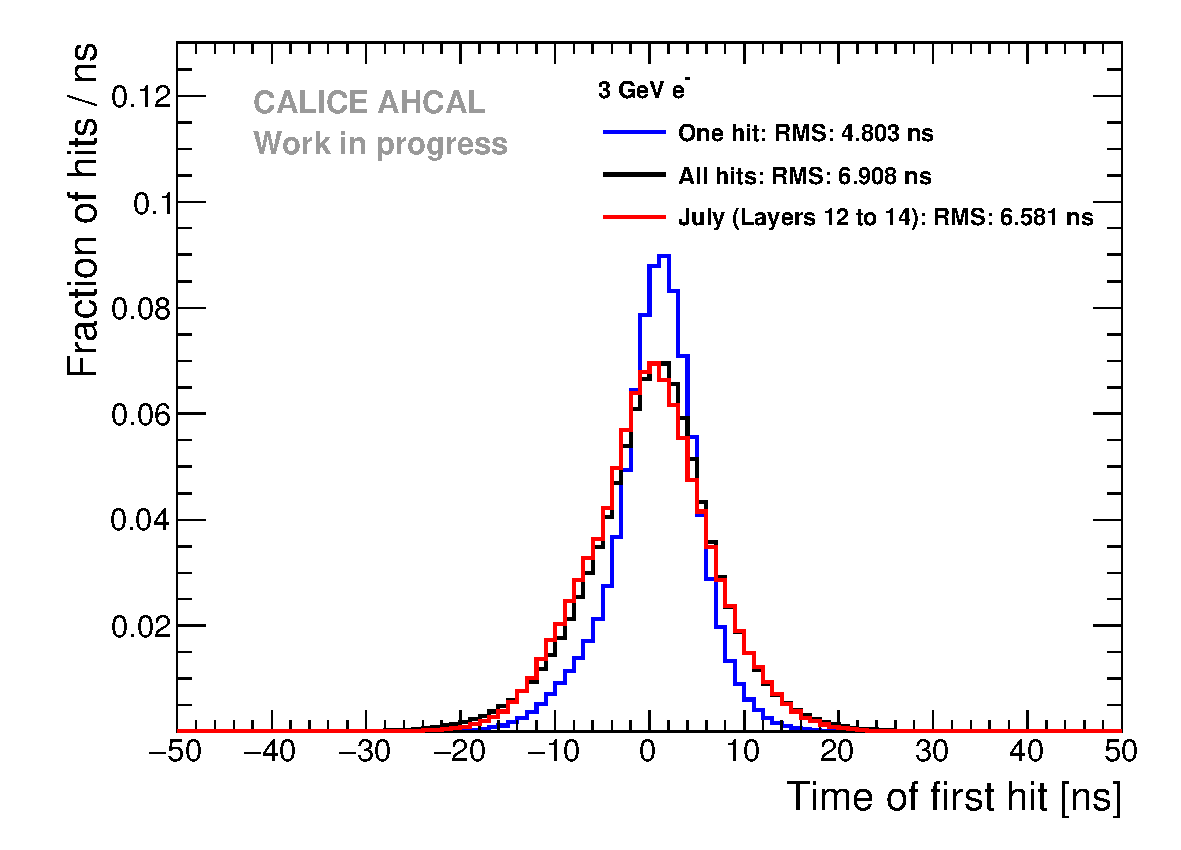
\includegraphics[width=0.6\textwidth]{../Thesis_Plots/Timing/Electrons/Plots/Timing_May2016_BigLayers.pdf}
	\caption{Time of the first hit distribution for 3 GeV electron showers at the DESY II testbeam in May 2016 combining layer 13 and 14. The blue distribution is the time of first hit in the case of events in which only single hits in a chip are taken.}\label{fig:TBMay2016}
\end{figure}

The figure \ref{fig:TBMay2016} shows the distribution of the time of first hits for layer 13 and 14 for all hits in black and for events with only single hits per chip in blue. The time resolution obtained of 6.8 ns is slightly better than the time resolution obtained at CERN in July 2015. The time distribution is narrower compared to the time distribution obtained at CERN. Similarly, the time distribution for events in which single hit per chip occurs is narrower by around 15\% compared to the muon time distribution. This is due to a lower number of hits per chip related to a lower beam energy. As well, it may be related to a different configuration of the time reference. Thus the width of the distribution is smaller with the effect observed in section \ref{subsec:ped_shift}.

We can learn from this study, that the time calibration constants determined in a specific dataset can also be used for another dataset with the same layers. Therefore, the timing calibration depends mainly on hardware and not so much on the environment.

\section{Systematic uncertainties}

For a significant assessment of differences observed between data and simulations, systematic uncertainties must be evaluated. Several possible sources were identified:

\begin{itemize}
	\item Non-Linearity correction: A non-linearity correction, as explained in section \ref{subsec:lin_corr}, determined from data with a limited accuracy lead to a systematic uncertainty. The residuals of the correction give a systematic error at the level of 0.2 ns.
	\item Time walk correction: Similarly to the non-linearity correction, the systematic error obtained from the residuals of the time walk correction (see section \ref{subsec:timewalk}) is in the order of 0.2 ns.
	\item Number of triggered channels correction: The correction for the number of triggered channels over 0.5 MIP in a chip results in a residual on the timing in the order of 1 ns. This systematic error is the most dominant over all other uncertainties.
	\item AHCAL energy scale: The energy scale of the AHCAL was determined using the muon dataset (see chapter \ref{chap:ECalibAHCAL}). A systematic uncertainty on the MIP scale of around 3.6\% was derived by dividing the muon sample in odd and even run numbers and by looking at the average spread of the fitted MIP value for both subsamples. This is converted to an uncertainty in time using the mean time of first hit as a function of the hit energy using the QGSP\_BERT\_HP physics list. At 0.5 MIP, this results in an uncertainty of 0.1 ns. For hits above 1 MIP, the uncertainty is below 0.05 ns.
	\item Time smearing parametrization: A parametrization was obtained from data for the width of the time smearing as a function of the number of triggered channels. An error band was obtained by comparing all electron energies as explained in appendix \ref{appendix:ped_shift}. This is applied to simulation for systematics.
	\item Determination of the offset to $t=0$: For simulation, the time shift per layer is calculated using a time of flight correction $T_{of} = \frac{z_{layer}}{c}$ with $c$ the speed of light and $z_{layer}$ the z position of a layer. For this, an uncertainty of 3 mm corresponding to the scintillator thickness is taken in z corresponding to 0.01 ns uncertainty in timing.
	\item Cross-talk: No measurement for optical cross-talk between tiles is available and from previous measurements, it varies between 10\% and 18\%. These are used for systematics in simulation only for the layers 4 to 10. The cross-talk value induces a different number of hits in the detector thus has an impact on the width of the time distribution.
	\item Detector inhomogeneities: As explained in section \ref{subsec:det_inhomo}, variations in the absolute number of entries in each time bin can be observed. The variations in the number of entries per time bin are between 10-20\%. Therefore a conservative uncertainty of 20\% on the data normalization is applied for the comparison of absolute number of hits per time bin.
	\item Absolute number of events: In the pion data, some possible contamination from multi-particle events may be present still after the selection as shown in section \ref{sec:pionsel}. Thus the number of absolute pion events is not known. Based on the time cluster time on simulation at the level of maximum 2\%, a 10\% uncertainty on the data normalization is assigned when comparing data to simulation for the absolute number of hits per time bin.
\end{itemize}

The systematic uncertainties are added in quadrature for the full systematic uncertainty. For comparison between data and simulation of the absolute time distribution, this results in an uncertainty of 20\% for muons/electrons and 30\% for pions on the data normalization. For the mean time of the first hit as a function of the hit energy and as a function of the distance to the shower center of gravity, the systematic uncertainty is resulting at 1.04 ns. The table \ref{table:time_syst} sums up the systematic uncertainties used in the analysis.
%% Systematics from number of hits may be underestimated... %
{
\renewcommand{\arraystretch}{1.2}
\begin{table}[htb!]
	\centering
	\caption{Summary of systematic uncertainties.}
	\label{table:time_syst}
	\begin{tabular}{@{} lc @{}}
		\toprule
		\multicolumn{1}{c}{Uncertainty source} & Full uncertainty steel \\
		\midrule
		Non-linearity residuals & 0.2 ns \\
		Time-walk residuals & 0.2 ns \\
		Number of triggered channels residuals & 1 ns \\
		Energy Scale & 0.05-0.1 ns \\
		Offset to $t=0$ & 0.01 ns (MC) \\
		Cross-talk & 10-18\% \\
		Detector inhomogeneities & 20\% \\
		Number of absolute events & 10\% (pions) \\
		\midrule
		\midrule
		\multicolumn{2}{c}{Systematics combined} \\
		\midrule
		data-MC hits per time bin & 20\% (muons/electrons) - 30\% (pions) \\
		data-MC vs hit energy & 1.09 ns \\
		data-MC vs hit distance to shower CoG & 1.09 ns \\
		\bottomrule
	\end{tabular}
\end{table}
}

\section{Validation of the simulation}

The simulation is validated by comparing the recorded muon and electron data to simulations. The timing resolution is extracted from muon data runs by fitting a double Gaussian to the data in the range [-50 ns, 50 ns] and is used to smear the timing of simulated calorimeter hits. The table \ref{table:time_res_sim} sums up the parameters used.

\begin{table}[htb!]
	\centering
	\caption{Timing resolution extracted with a double Gaussian fit from muon data used for simulation.}
	\label{table:time_res_sim}
	\begin{tabular}{@{} cccccc @{}}
		\hline
		$\alpha_{1}$ & $\mu_{1}$ [ns] & $\sigma_{1}$ [ns] & $\alpha_{2}$ & $\mu_{2}$ [ns] & $\sigma_{2}$ [ns] \\
		\hline
		0.607352 & -0.699093 & 5.85891 & 0.391041 & 0.945272 & 3.4012 \\
		\hline
	\end{tabular}
\end{table}

The comparison of the time of first hit distribution for muons is shown in figure \ref{fig:sim_data_muon}. The large uncertainties observed in the simulation are due to the systematics of the different cross-talk values. The comparison shows that in the range of -20 ns to 20 ns, the data and simulation agree well within the uncertainties. However, over 20 ns (respectively below -20 ns), the tails of the simulation don't agree with data. This is due to the noise implementation in simulation that is not perfectly reproduced and that is suppressed by the track finder selection.

\begin{figure}[htbp!]
	\centering
	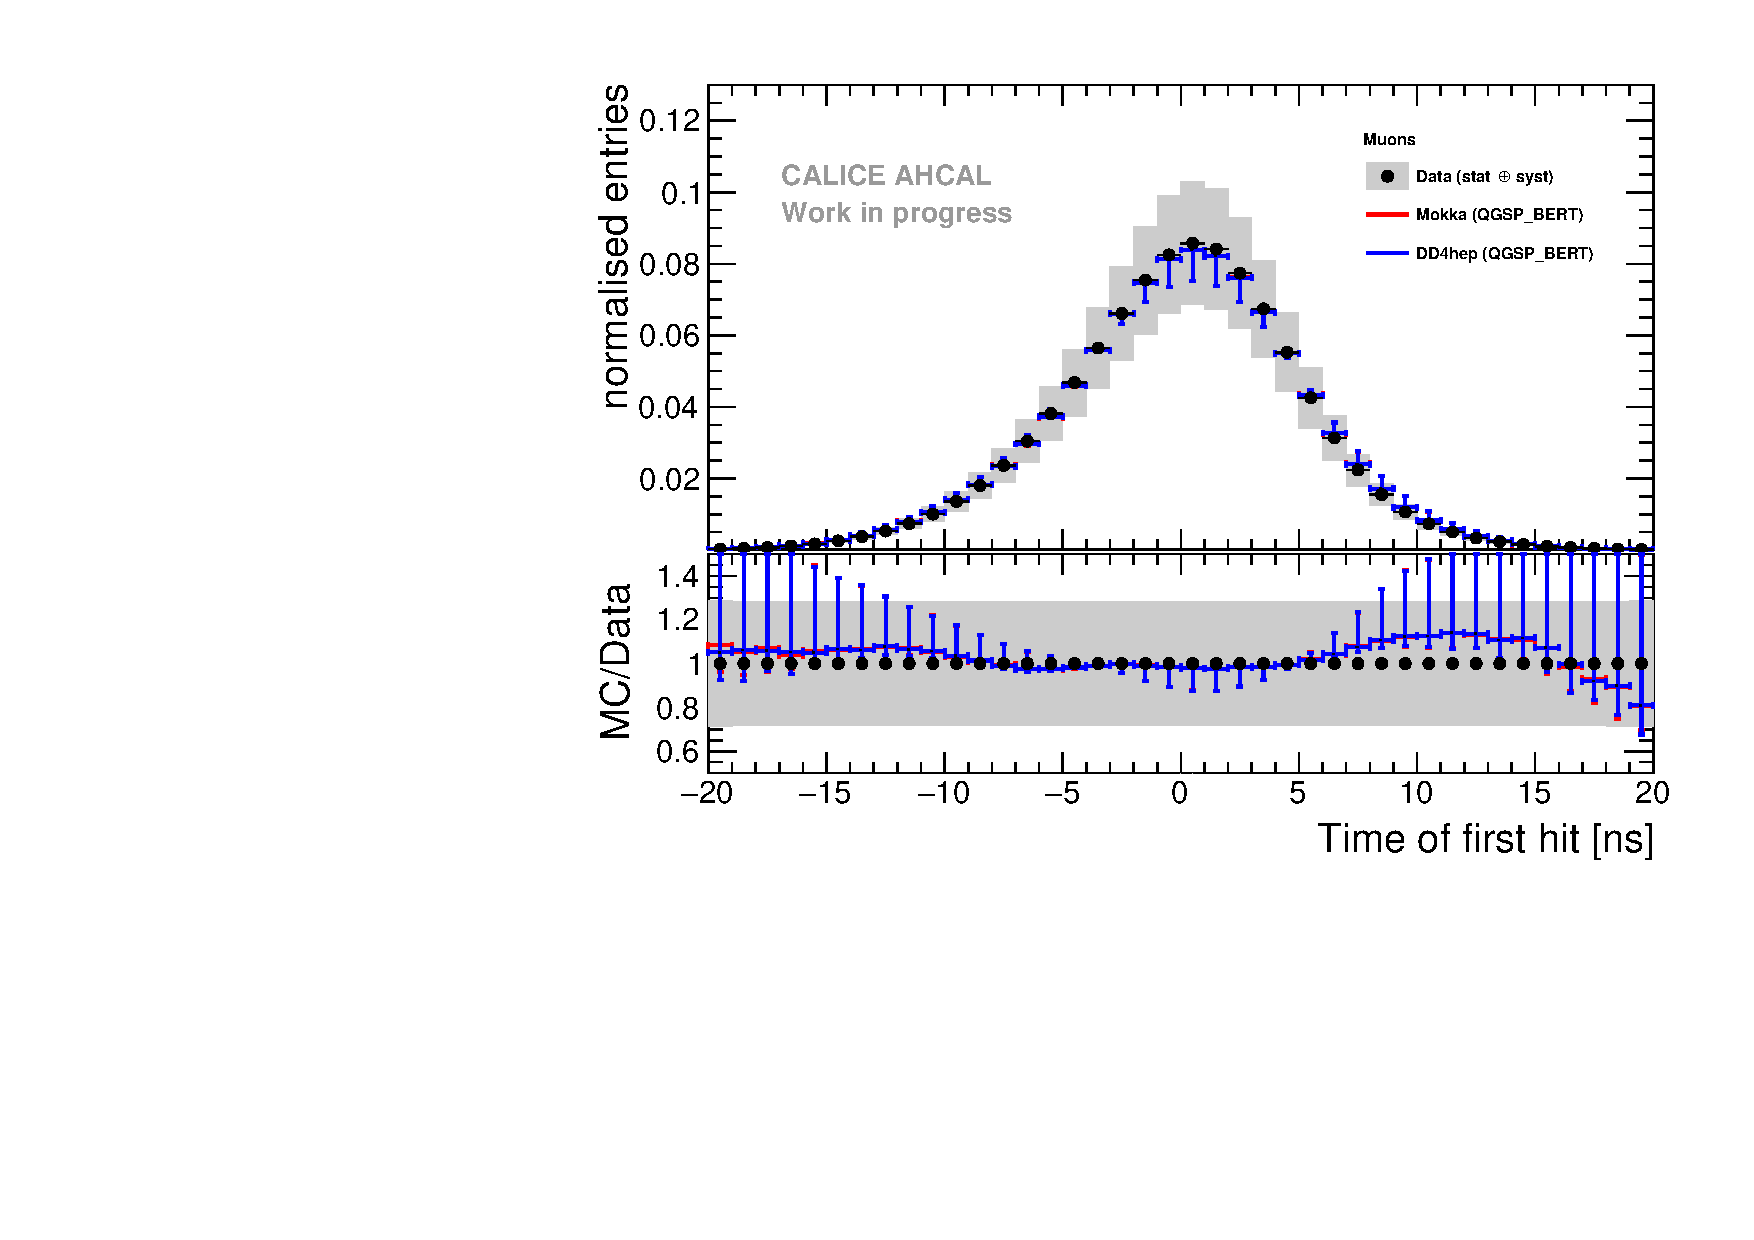
\includegraphics[width=0.7\textwidth]{../Thesis_Plots/Timing/Muons/Plots/Comparison_MokkaDD4hepData_Muons.pdf}
	\caption{Time of first hit distribution for muons in data and simulation between -30 and 30 ns. The grey area represents the statistic and systematic uncertainty of the data. The error bars of the simulation are obtained by varying the cross-talk parameter between 10\% and 18\%.}
	\label{fig:sim_data_muon}
\end{figure}

To further validate the simulation, comparisons with electron data is necessary. In addition to the muon resolution, a parametrization of the increase of the width of the time distribution as a function of the number of triggered channels in a chip above 0.5 MIPs is added in simulation as described in appendix \ref{appendix:ped_shift}. The figure \ref{fig:elec_sim_data_10GeV} shows the comparison of the time of first hit distribution for 10 GeV electrons. The errors bars in the simulation is obtained by varying the cross-talk parameter between 10\% and 18\% and from the uncertainty on the time smearing parametrization which is dominant. The time distributions and the distribution of the number of triggered channels per chip have been checked for all energies and they can be seen in appendix \ref{appendix:TimingAdd}.

\begin{figure}[htbp!]
	\centering
	\begin{subfigure}[t]{0.49\textwidth}
		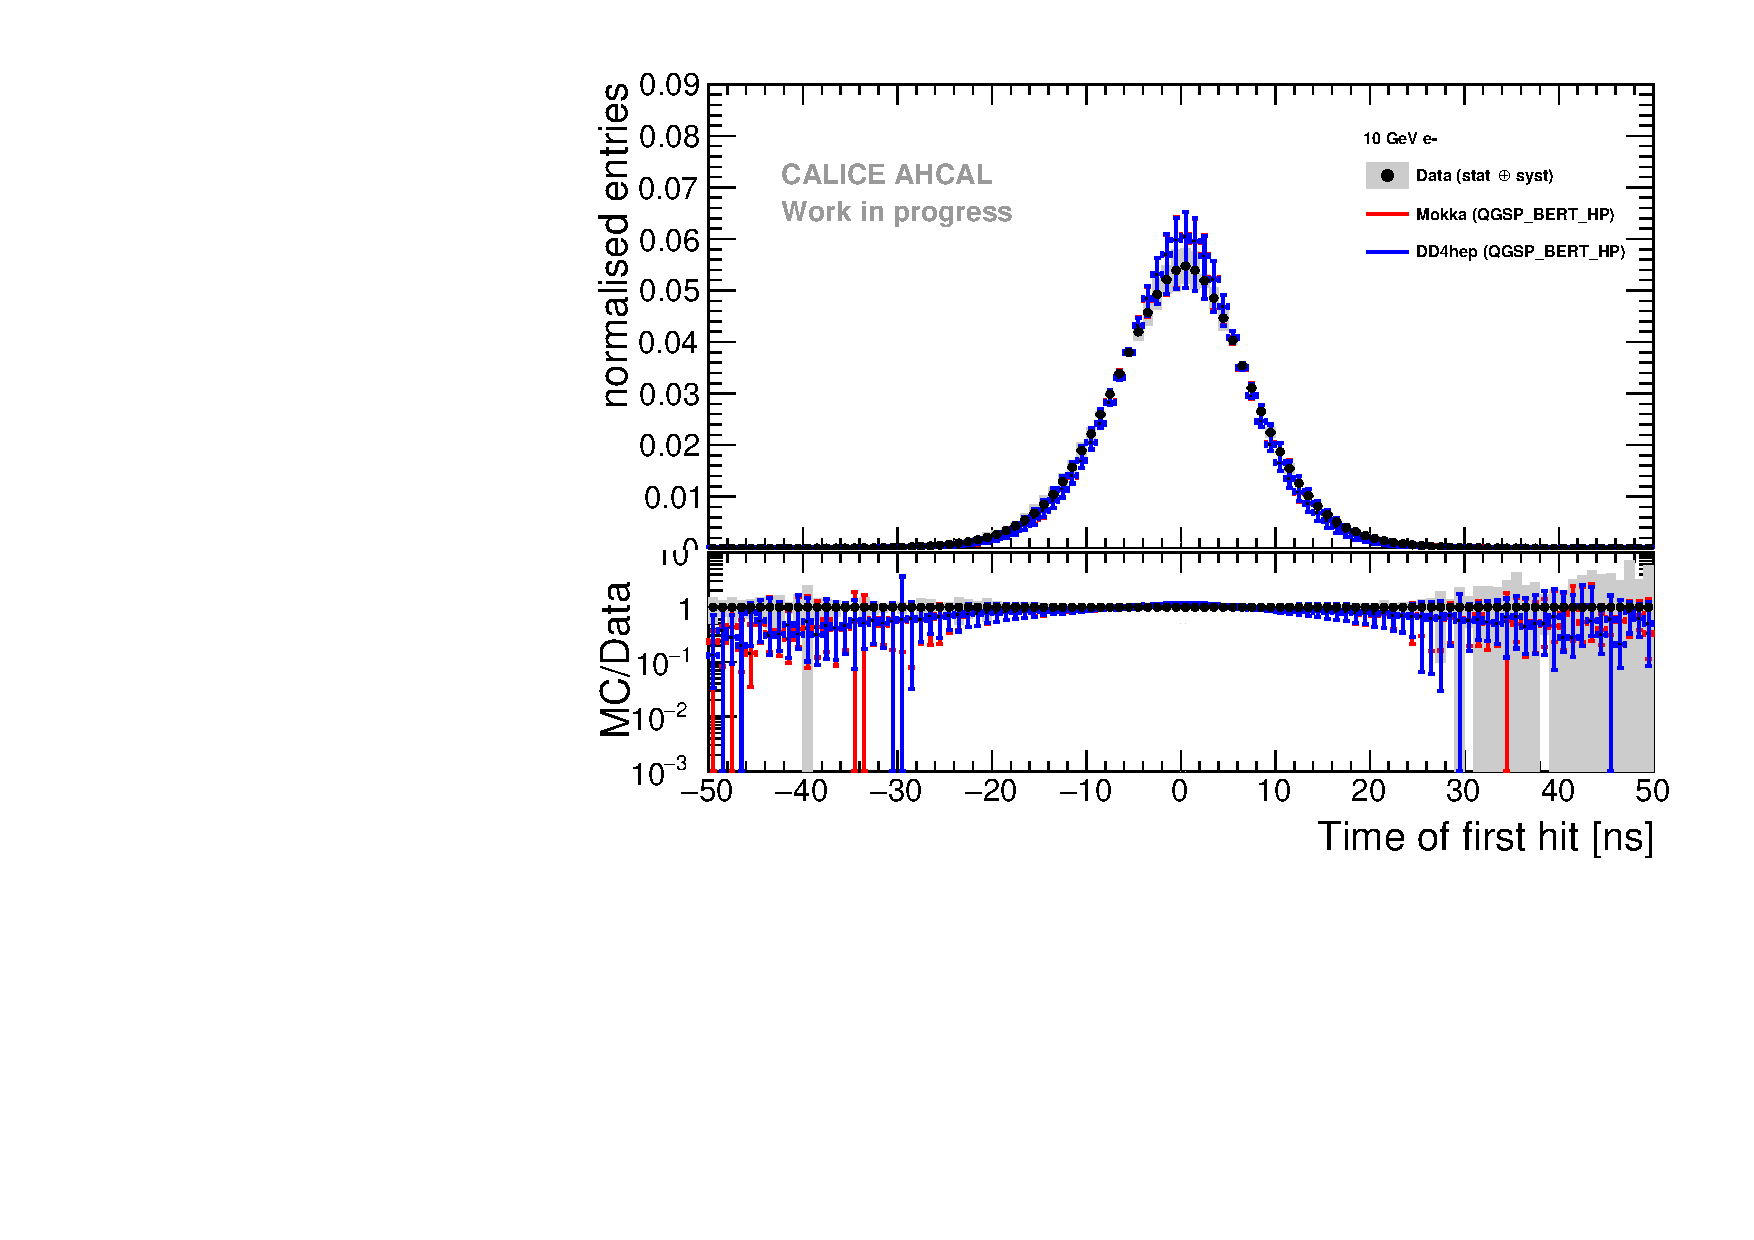
\includegraphics[width=1\textwidth]{../Thesis_Plots/Timing/Electrons/Plots/Comparison_SimData_Electrons10GeV.pdf}
		\caption{}\label{fig:elec_sim_data_10GeV}
	\end{subfigure}
	\hfill
	\begin{subfigure}[t]{0.49\textwidth}
		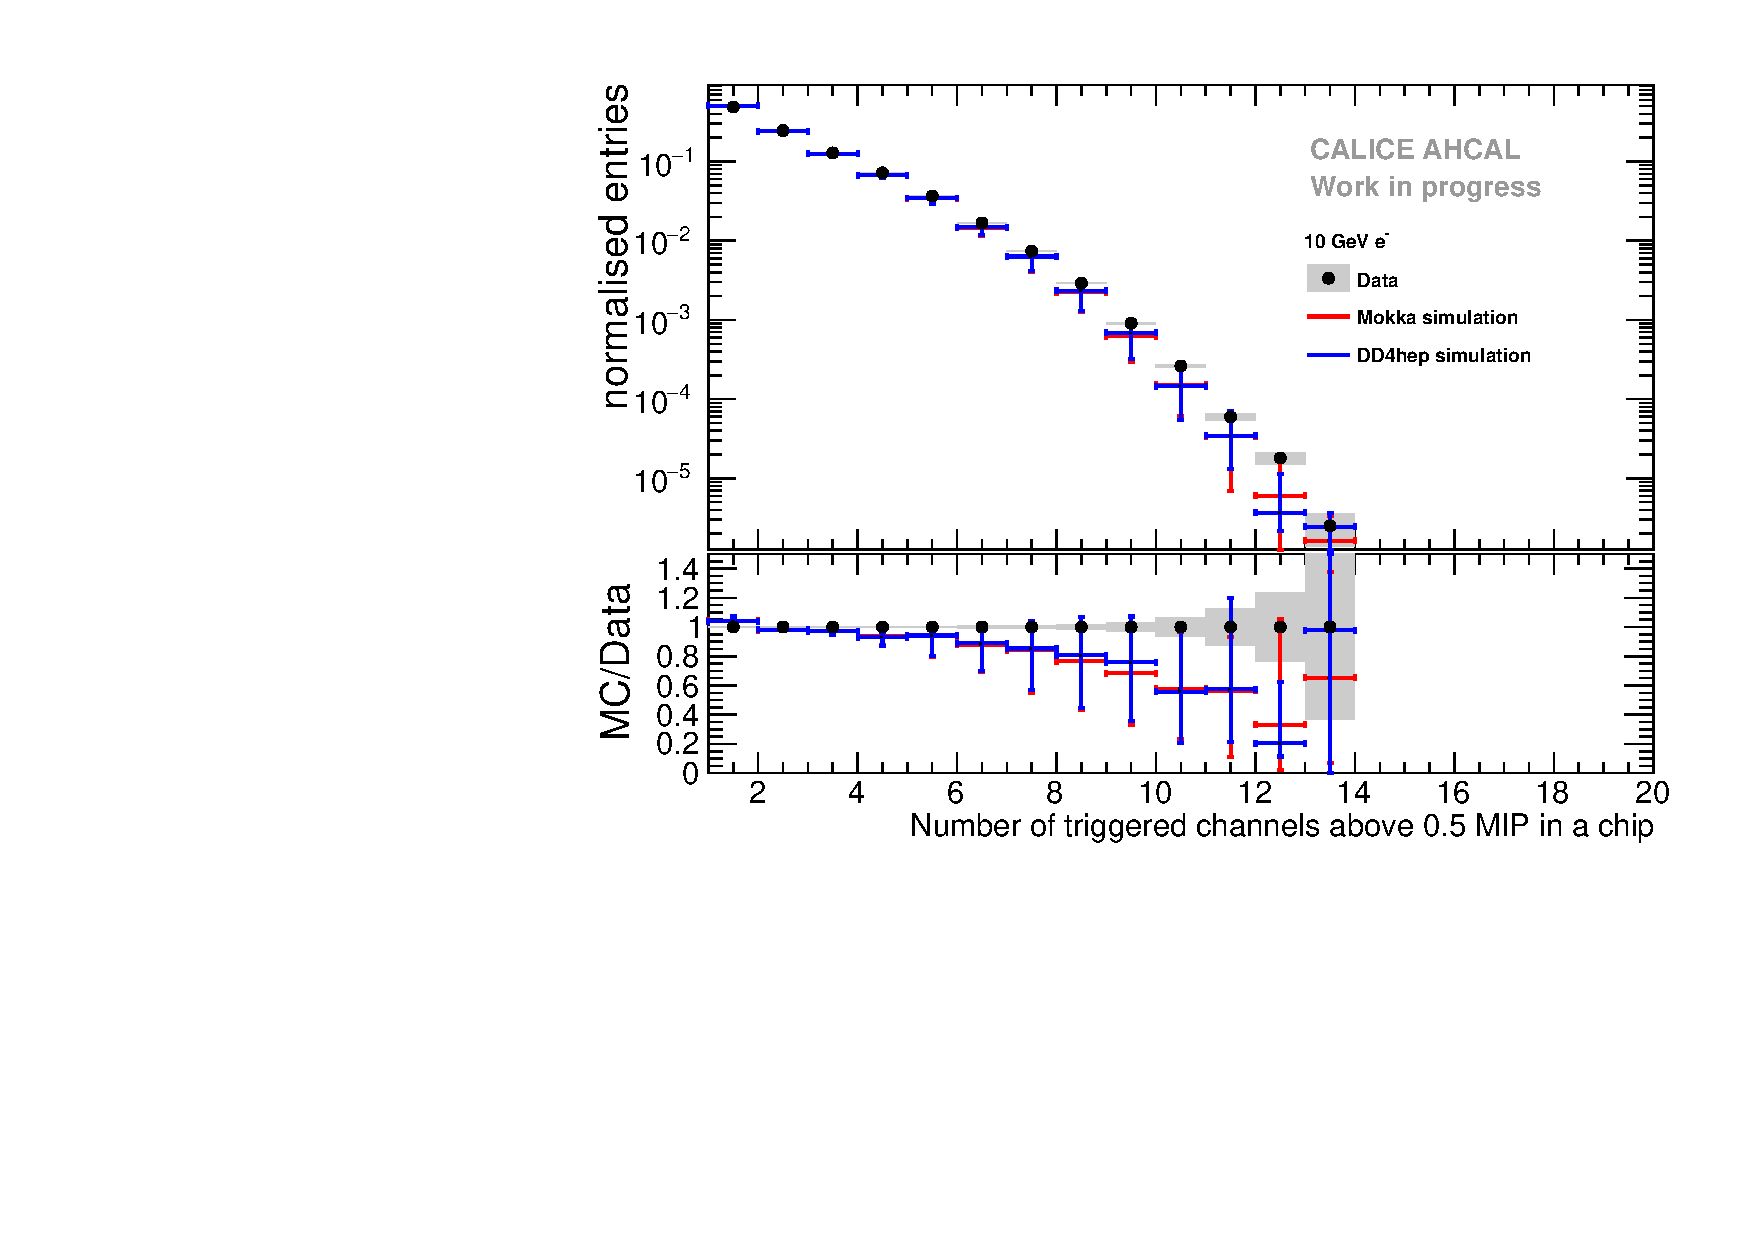
\includegraphics[width=1\textwidth]{../Thesis_Plots/Timing/Electrons/Plots/Comparison_SimData_Electrons_nHits_10GeV.pdf}
		\caption{}\label{fig:elec_sim_data_nHits_10GeV}
	\end{subfigure}
	\caption{\subref{fig:elec_sim_data_10GeV}) Comparison of the time of first hit between data and simulations for 10 GeV electrons. The grey area represents the statistical and systematical error of the data. Error bars in simulation are obtained by varying the cross-talk parameter between 10\% and 10\% and with the uncertainty on the time smearing parametrization. \subref{fig:elec_sim_data_nHits_10GeV}) Comparison of the number of triggered channels per chip between data and MC for 10 GeV electrons. The grey area represents the statistical error of the data. Error bars in simulation are obtained by varying the cross-talk parameter between 10\% and 18\%.}
\end{figure}

The simulation is systematically narrower than data. This is caused by the simulation having fewer hits per chip than data which can be seen in figure \ref{fig:elec_sim_data_nHits_10GeV}. The simulation is generally 10\% to 20\% lower than data in the region of 6 to 10 hits per chip.

For the distributions of the time of first hit, the simulation agrees best at 10 and 20 GeV in the central region of -15 ns to 15 ns. At higher energies, the simulation overestimate slightly in the region of 10-20 ns similarly in the region -10 ns to -20 ns. This may come from imperfect beam profiles where a slight shift in the simulation can influence highly the number of triggered channels in a chip. In addition, the number of triggered channels parametrization may be imperfect. But due to the limited amount of data, only a global parametrization could be applied.

For all energies, the description of the tails of the time of first hit distribution in the simulation that well are underestimated. This is due to the description of the noise in the simulation that is not perfectly reproduced. Overall, the simulation describes well the data within statistical and systematic uncertainties in the central region.

\begin{center}
	\rule{0.5\textwidth}{.4pt}
\end{center}

In this chapter, the timing analysis of the recorded electron data has been presented. A time resolution between 7.8 ns at 10 GeV beam energy and 8.5 ns at 50 GeV beam energy. An increase of the width of the time distribution as a function of the number of triggered channels in a chip is seen in the electron data. This increase of the time resolution is used as an input to tune the simulation in order to describe the data.

The AHCAL timing simulation has been validated by comparing the simulated time distributions to data using muons and electrons. Overall, the simulation reproduces the data within 20\% in the range of -30 ns to 30 ns. However, the simulation underestimates highly the tails of the distribution that is due to an imperfect implementation of noise hits in the simulation.

The simulation is in good enough agreement with data that the time of hadron showers can be studied. In the next chapter, the timing analysis of pion showers and comparisons to simulation will be presented.
